% ============================================================
%  Fig. 1  Mechanism-level SHAP audit pipeline (full width, figure*)
%  Compile standalone:  pdflatex audit_pipeline.tex
%  Then in the paper:   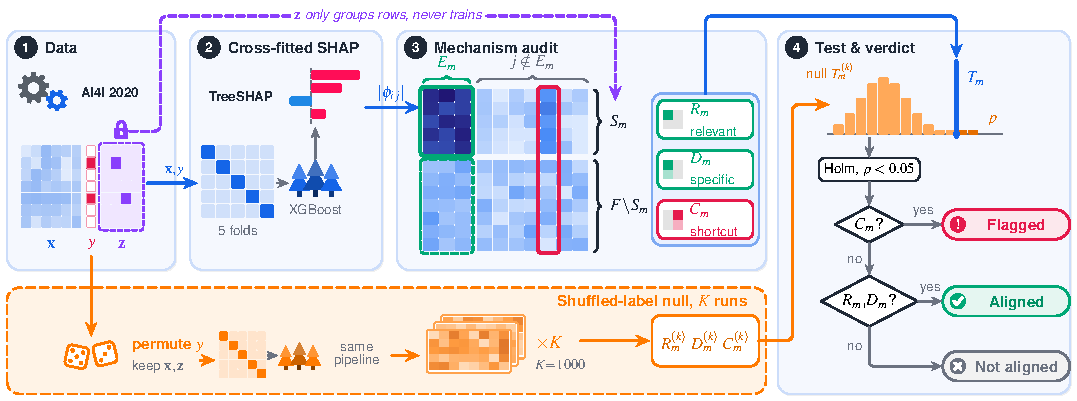
\includegraphics[width=\textwidth]{audit_pipeline.pdf}
%  Built at 18 cm wide, so it drops into IEEE \textwidth (7.16 in) at ~1:1.
%  No icon packages needed: every icon is drawn in plain TikZ.
% ============================================================
\documentclass[tikz,border=3pt]{standalone}
\usepackage[T1]{fontenc}
\usepackage{mathptmx}
\usepackage[scaled=0.92]{helvet}
\renewcommand{\familydefault}{\sfdefault}
\usepackage{amsmath}
\usetikzlibrary{calc,arrows.meta,decorations.pathreplacing,shapes.geometric,shadows}

% ---------------- palette (vivid, colour-blind aware) ----------------
\definecolor{obs}{HTML}{1565E8}    % observed labels
\definecolor{obsL}{HTML}{EAF1FF}
\definecolor{nul}{HTML}{FF7A00}    % permuted labels (null)
\definecolor{nulL}{HTML}{FFF3E6}
\definecolor{trig}{HTML}{00A876}   % expected trigger features E_m
\definecolor{cut}{HTML}{E5194B}    % shortcut / failure
\definecolor{flag}{HTML}{8A3FFC}   % mechanism flags z
\definecolor{ink}{HTML}{1F2937}
\definecolor{mute}{HTML}{6B7280}
\definecolor{panel}{HTML}{F5F8FE}
\definecolor{shapR}{HTML}{FF0D57}  % SHAP library red
\definecolor{shapB}{HTML}{1E88E5}  % SHAP library blue
\definecolor{hA}{HTML}{EDF4FF}     % heat ramp, observed
\definecolor{hB}{HTML}{4A8CF7}
\definecolor{hC}{HTML}{1F1270}
\definecolor{nA}{HTML}{FFF1E2}     % heat ramp, null
\definecolor{nB}{HTML}{FF9B40}
\definecolor{nC}{HTML}{A33000}

% ---------------- styles ----------------
\tikzset{
  panelbox/.style={rounded corners=6pt, fill=panel, draw=obs!22, line width=0.6pt,
                   drop shadow={opacity=0.12, shadow xshift=0.6pt, shadow yshift=-0.8pt}},
  num/.style={circle, fill=ink, text=white, font=\sffamily\bfseries\scriptsize,
              inner sep=0pt, minimum size=3.8mm},
  ptitle/.style={font=\sffamily\bfseries\footnotesize, text=ink, anchor=west},
  flow/.style={-{Stealth[length=2.3mm,width=1.9mm]}, line width=1.1pt, rounded corners=3pt},
  thin/.style={-{Stealth[length=1.7mm,width=1.4mm]}, line width=0.8pt, draw=mute, rounded corners=2pt},
  lbl/.style={font=\sffamily\scriptsize, text=mute},
  badge/.style={rounded corners=7pt, line width=0.9pt, minimum height=0.5cm,
                minimum width=2.15cm, font=\sffamily\bfseries\footnotesize,
                inner xsep=4pt, text depth=0pt, align=center},
  dia/.style={diamond, aspect=1.9, draw=ink, line width=0.8pt, fill=white,
              inner sep=1.2pt, font=\footnotesize},
}

% ---------------- helpers ----------------
% \heat{value 0..1}{low}{mid}{high}  -> defines colour "hc"
\newcommand{\heat}[4]{%
  \pgfmathsetmacro{\hv}{#1}%
  \pgfmathtruncatemacro{\hb}{\hv<0.5 ? 1 : 0}%
  \ifnum\hb=1
    \pgfmathtruncatemacro{\hp}{200*\hv}\colorlet{hc}{#3!\hp!#2}%
  \else
    \pgfmathtruncatemacro{\hp}{200*(\hv-0.5)}\colorlet{hc}{#4!\hp!#3}%
  \fi}

% gear icon \gear{x}{y}{radius}{teeth}{colour}
\newcommand{\gear}[5]{%
  \begin{scope}[shift={(#1,#2)}]
    \pgfmathsetmacro{\gi}{#3*0.76}\pgfmathsetmacro{\gs}{360/#4}
    \fill[#5] (0:\gi) \foreach \k in {1,...,#4}{
        -- ({(\k-1)*\gs+\gs*0.12}:#3) -- ({(\k-1)*\gs+\gs*0.45}:#3)
        -- ({(\k-1)*\gs+\gs*0.57}:\gi) -- ({\k*\gs}:\gi)} -- cycle;
    \fill[panel] (0,0) circle ({#3*0.34});
  \end{scope}}

% small pine-tree icon \tree{x}{ybase}{colour}{scale}
\newcommand{\treeicon}[4]{%
  \begin{scope}[shift={(#1,#2)}, scale=#4]
    \fill[#3!55!black] (-0.03,0) rectangle (0.03,0.1);
    \fill[#3] (0,0.40) -- (-0.17,0.10) -- (0.17,0.10) -- cycle;
    \fill[#3!80!white] (0,0.54) -- (-0.12,0.30) -- (0.12,0.30) -- cycle;
  \end{scope}}

% padlock \lock{x}{y}{colour}
\newcommand{\lockicon}[3]{%
  \begin{scope}[shift={(#1,#2)}]
    \draw[#3, line width=1.1pt] (-0.06,0.15) -- (-0.06,0.22) arc (180:0:0.06) -- (0.06,0.15);
    \fill[#3, rounded corners=0.6pt] (-0.11,0) rectangle (0.11,0.17);
    \fill[white] (0,0.085) circle (0.022);
  \end{scope}}

% die \die{x}{y}{angle}{colour}{pips 3|5}
\newcommand{\die}[5]{%
  \begin{scope}[shift={(#1,#2)}, rotate=#3]
    \filldraw[fill=white, draw=#4, line width=0.9pt, rounded corners=2pt]
      (-0.18,-0.18) rectangle (0.18,0.18);
    \ifnum#5=5
      \foreach \p in {(-0.09,-0.09),(0.09,0.09),(-0.09,0.09),(0.09,-0.09),(0,0)}
        \fill[#4] \p circle (0.03);
    \else
      \foreach \p in {(-0.09,-0.09),(0,0),(0.09,0.09)} \fill[#4] \p circle (0.03);
    \fi
  \end{scope}}

% 5x5 cross-fitting grid, top-left (x,y), cell size, colour
\newcommand{\foldgrid}[4]{%
  \foreach \fr in {1,...,5}{\foreach \fc in {1,...,5}{
    \ifnum\fr=\fc \colorlet{fg}{#4}\else\colorlet{fg}{#4!20}\fi
    \fill[fg, rounded corners=0.6pt]
      ({#1+(\fc-1)*#3},{#2-(\fr-1)*#3}) rectangle ++({#3*0.86},{-#3*0.86});
  }}}

% unstructured mini heat-map for null copies: top-left (x,y), seed
\newcommand{\miniheat}[3]{%
  \pgfmathsetseed{#3}%
  \fill[white, draw=nul!70, line width=0.5pt, rounded corners=1pt]
    ({#1-0.04},{#2+0.04}) rectangle ({#1+8*0.17+0.02},{#2-5*0.13-0.04});
  \foreach \mr in {1,...,5}{\foreach \mc in {1,...,8}{
    \pgfmathsetmacro{\mu}{0.12+0.55*rnd}\heat{\mu}{nA}{nB}{nC}%
    \fill[hc] ({#1+(\mc-1)*0.17},{#2-(\mr-1)*0.13}) rectangle ++(0.15,-0.11);
  }}}

% =====================================================================
\begin{document}
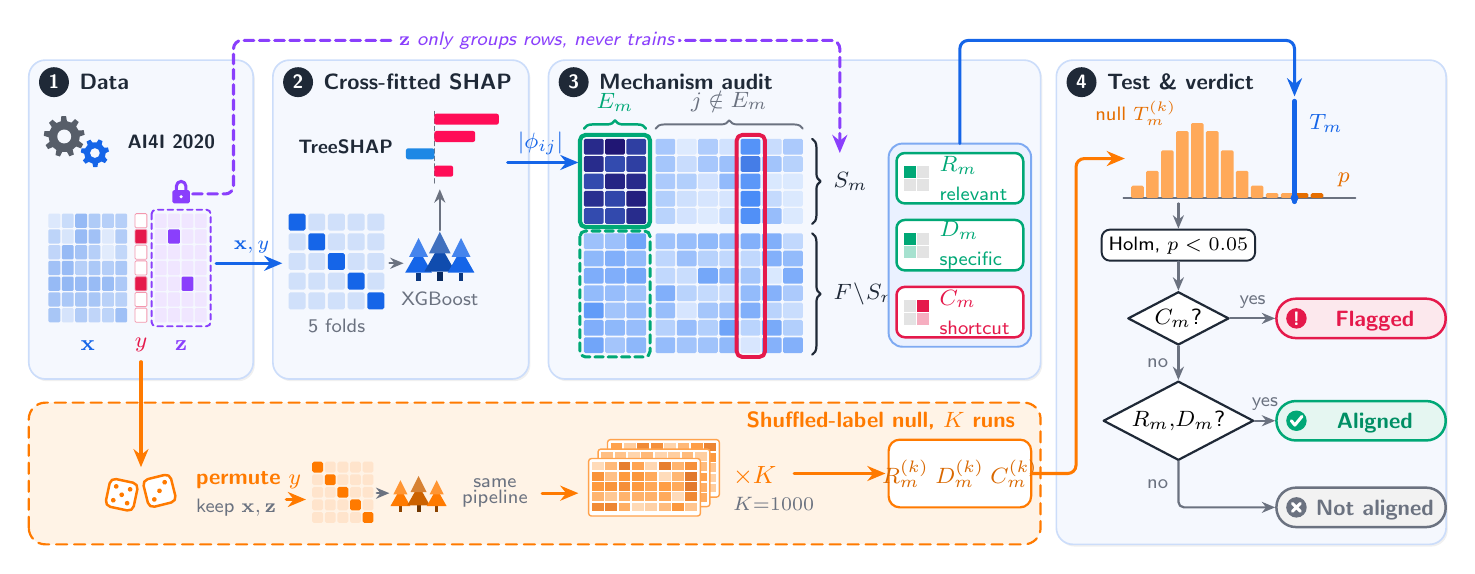
\begin{tikzpicture}[line cap=round, line join=round]

% ---------------- panels ----------------
\path[panelbox] (0,2.25) rectangle (2.85,6.3);
\path[panelbox] (3.1,2.25) rectangle (6.35,6.3);
\path[panelbox] (6.6,2.25) rectangle (12.85,6.3);
\path[panelbox] (13.05,0.15) rectangle (18.0,6.3);
\filldraw[fill=nulL, draw=nul, line width=0.8pt, dash pattern=on 4pt off 2.5pt,
          rounded corners=6pt] (0,0.15) rectangle (12.85,1.95);

\node[num] at (0.32,6.02) {1};  \node[ptitle] at (0.52,6.02) {Data};
\node[num] at (3.42,6.02) {2};  \node[ptitle] at (3.62,6.02) {Cross-fitted SHAP};
\node[num] at (6.92,6.02) {3};  \node[ptitle] at (7.12,6.02) {Mechanism audit};
\node[num] at (13.37,6.02) {4}; \node[ptitle] at (13.57,6.02) {Test \& verdict};
\node[font=\sffamily\bfseries\footnotesize, text=nul, anchor=east] at (12.65,1.72)
      {Shuffled-label null, $K$ runs};

% =====================================================================
% (1) DATA
\gear{0.45}{5.33}{0.26}{9}{ink!75}
\gear{0.84}{5.12}{0.18}{7}{obs}
\node[font=\sffamily\bfseries\scriptsize, text=ink, anchor=west] at (1.13,5.26) {AI4I 2020};

\pgfmathsetseed{3}
\foreach \tr in {1,...,7}{
  \foreach \tc in {1,...,6}{                                   % sensors x
    \pgfmathtruncatemacro{\sh}{12+35*rnd}
    \fill[obs!\sh, rounded corners=0.4pt]
      ({0.25+(\tc-1)*0.17},{4.35-(\tr-1)*0.2}) rectangle ++(0.15,-0.18);}
  \pgfmathtruncatemacro{\isf}{(\tr==2 || \tr==5) ? 1 : 0}       % label y
  \ifnum\isf=1 \colorlet{yc}{cut}\else\colorlet{yc}{white}\fi
  \filldraw[fill=yc, draw=cut!45, line width=0.3pt, rounded corners=0.4pt]
      (1.35,{4.35-(\tr-1)*0.2}) rectangle ++(0.15,-0.18);
  \foreach \tc in {1,...,4}{                                   % flags z
    \pgfmathtruncatemacro{\on}{((\tr==2 && \tc==2) || (\tr==5 && \tc==3)) ? 1 : 0}
    \ifnum\on=1 \colorlet{zc}{flag}\else\colorlet{zc}{flag!13}\fi
    \fill[zc, rounded corners=0.4pt]
      ({1.6+(\tc-1)*0.17},{4.35-(\tr-1)*0.2}) rectangle ++(0.15,-0.18);}
}
\draw[flag, line width=0.7pt, dash pattern=on 2pt off 1.5pt, rounded corners=1.5pt]
     (1.56,4.4) rectangle (2.31,2.92);
\lockicon{1.935}{4.48}{flag}
\node[font=\footnotesize, text=obs]  at (0.75,2.68) {$\mathbf{x}$};
\node[font=\footnotesize, text=cut]  at (1.425,2.68) {$y$};
\node[font=\footnotesize, text=flag] at (1.935,2.68) {$\mathbf{z}$};

% flags travel above the panels and only touch the row grouping
\draw[flow, flag, dash pattern=on 3.5pt off 2pt]
     (2.08,4.6) -- (2.6,4.6) -- (2.6,6.55) -- (10.3,6.55) -- (10.3,5.12);
\node[font=\sffamily\itshape\scriptsize, text=flag, fill=white, inner sep=1.5pt,
      rounded corners=2pt] at (6.45,6.55) {$\mathbf{z}$ only groups rows, never trains};

% =====================================================================
% (2) CROSS-FITTED SHAP
\draw[flow, obs] (2.38,3.72) -- (3.22,3.72);
\node[font=\scriptsize, text=obs] at (2.83,3.92) {$\mathbf{x},y$};

\foldgrid{3.3}{4.35}{0.25}{obs}
\node[lbl] at (3.91,2.92) {5 folds};
\draw[thin] (4.58,3.72) -- (4.76,3.72);
\treeicon{4.95}{3.5}{obs}{1}
\treeicon{5.22}{3.5}{obs!75!black}{1.15}
\treeicon{5.49}{3.5}{obs}{1}
\node[lbl] at (5.22,3.27) {XGBoost};
\draw[thin] (5.22,4.14) -- (5.22,4.66);

% SHAP explanation glyph (library colours)
\draw[mute, line width=0.5pt, dash pattern=on 1.5pt off 1.2pt] (5.15,4.74) -- (5.15,5.68);
\foreach \v/\c [count=\i] in {0.82/shapR, 0.52/shapR, -0.36/shapB, 0.24/shapR}{
  \fill[\c, rounded corners=0.8pt] (5.15,{5.62-(\i-1)*0.22}) rectangle ++(\v,-0.14);}
\node[font=\sffamily\bfseries\scriptsize, text=ink, anchor=west] at (3.3,5.2) {TreeSHAP};

\draw[flow, obs] (6.08,5.0) -- (6.98,5.0);
\node[font=\footnotesize, text=obs] at (6.5,5.24) {$|\phi_{ij}|$};

% =====================================================================
% (3) MECHANISM AUDIT : the |phi| matrix
\def\mx{7.05}\def\my{5.3}\def\cw{0.27}\def\ch{0.22}
\pgfmathsetseed{11}
\foreach \row in {1,...,12}{
  \foreach \col in {1,...,10}{
    \pgfmathsetmacro{\u}{rnd}
    \ifnum\row<6
      \ifnum\col<4 \pgfmathsetmacro{\v}{0.72+0.28*\u}
      \else\ifnum\col=8 \pgfmathsetmacro{\v}{0.40+0.18*\u}
      \else \pgfmathsetmacro{\v}{0.04+0.26*\u}\fi\fi
    \else
      \ifnum\col<4 \pgfmathsetmacro{\v}{0.22+0.24*\u}
      \else \pgfmathsetmacro{\v}{0.06+0.34*\u}\fi
    \fi
    \heat{\v}{hA}{hB}{hC}
    \pgfmathsetmacro{\gx}{\col>3 ? 0.1 : 0}
    \pgfmathsetmacro{\gy}{\row>5 ? 0.1 : 0}
    \fill[hc, rounded corners=0.5pt]
      ({\mx+(\col-1)*\cw+\gx},{\my-(\row-1)*\ch-\gy}) rectangle ++(0.25,-0.20);
}}
% block highlights
\draw[trig, line width=1.5pt, rounded corners=2pt] (7.0,5.35) rectangle (7.89,4.18);
\draw[trig, line width=1.1pt, rounded corners=2pt, dash pattern=on 3pt off 1.8pt]
     (7.0,4.13) rectangle (7.89,2.53);
\draw[cut, line width=1.4pt, rounded corners=2pt] (8.99,5.35) rectangle (9.35,2.53);

% braces
\draw[decorate, decoration={brace, amplitude=3pt}, trig, line width=0.9pt]
     (7.05,5.43) -- (7.84,5.43) node[midway, above=2.5pt, font=\footnotesize, text=trig] {$E_m$};
\draw[decorate, decoration={brace, amplitude=3pt}, mute, line width=0.7pt]
     (7.96,5.43) -- (9.83,5.43) node[midway, above=2.5pt, font=\footnotesize, text=mute] {$j\notin E_m$};
\draw[decorate, decoration={brace, amplitude=3pt}, ink, line width=0.8pt]
     (9.95,5.3) -- (9.95,4.22) node[midway, right=4pt, font=\footnotesize, text=ink] {$S_m$};
\draw[decorate, decoration={brace, amplitude=3pt}, ink, line width=0.8pt]
     (9.95,4.1) -- (9.95,2.56) node[midway, right=4pt, font=\footnotesize, text=ink] {$F\!\setminus\! S_m$};

% observed statistic chips
\filldraw[fill=obsL, draw=obs!55, line width=0.7pt, rounded corners=5pt]
     (10.92,2.66) rectangle (12.73,5.24);
\foreach \yc/\name/\word/\col/\kind in
   {4.8/R_m/relevant/trig/1, 3.95/D_m/specific/trig/2, 3.1/C_m/shortcut/cut/3}{
  \filldraw[fill=white, draw=\col, line width=0.9pt, rounded corners=3pt]
     (11.02,\yc-0.32) rectangle (12.63,\yc+0.32);
  % 2x2 glyph: rows (S_m, F\S_m) x cols (E_m, others)
  \foreach \gr/\gc in {0/0,0/1,1/0,1/1}
     \fill[gray!22] ({11.12+\gc*0.165},{\yc+0.15-\gr*0.165}) rectangle ++(0.145,-0.145);
  \ifnum\kind=1 \fill[trig] (11.12,\yc+0.15) rectangle ++(0.145,-0.145); \fi
  \ifnum\kind=2 \fill[trig] (11.12,\yc+0.15) rectangle ++(0.145,-0.145);
                \fill[trig!35] (11.12,\yc-0.015) rectangle ++(0.145,-0.145); \fi
  \ifnum\kind=3 \fill[cut] (11.285,\yc+0.15) rectangle ++(0.145,-0.145);
                \fill[cut!35] (11.285,\yc-0.015) rectangle ++(0.145,-0.145); \fi
  \node[anchor=west, align=left, inner sep=0pt, text=\col] at (11.56,\yc)
       {{\footnotesize$\name$}\\[-1.5pt]{\sffamily\scriptsize \word}};
}

% =====================================================================
% NULL LANE
\draw[flow, nul] (1.425,2.47) -- (1.425,1.13);
\die{1.18}{0.78}{-12}{nul}{5}
\die{1.66}{0.83}{14}{nul}{3}
\node[font=\sffamily\bfseries\footnotesize, text=nul, anchor=west] at (2.0,0.97) {permute $y$};
\node[lbl, anchor=west] at (2.0,0.62) {keep $\mathbf{x},\mathbf{z}$};

\draw[flow, nul] (3.27,0.72) -- (3.52,0.72);
\foldgrid{3.6}{1.2}{0.16}{nul}
\draw[thin] (4.42,0.8) -- (4.58,0.8);
\treeicon{4.72}{0.56}{nul}{0.75}
\treeicon{4.95}{0.56}{nul!80!black}{0.85}
\treeicon{5.18}{0.56}{nul}{0.75}
\node[lbl, align=center] at (5.92,0.8) {same\\[-2pt]pipeline};

\draw[flow, nul] (6.52,0.8) -- (6.98,0.8);
\miniheat{7.39}{1.44}{21}
\miniheat{7.27}{1.32}{22}
\miniheat{7.15}{1.20}{23}
\node[font=\sffamily\bfseries\small, text=nul, anchor=west] at (8.82,1.02) {$\times K$};
\node[lbl, anchor=west] at (8.82,0.66) {$K{=}1000$};

\draw[flow, nul] (9.72,1.05) -- (10.88,1.05);
\filldraw[fill=white, draw=nul, line width=0.8pt, rounded corners=4pt]
     (10.92,0.62) rectangle (12.73,1.48);
\node[font=\footnotesize, text=nul!85!black] at (11.825,1.05)
     {$R^{(k)}_m\; D^{(k)}_m\; C^{(k)}_m$};

% =====================================================================
% (4) TEST & VERDICT
% null histogram
\draw[mute, line width=0.5pt] (13.9,4.55) -- (16.85,4.55);
\foreach \i in {1,...,13}{
  \pgfmathsetmacro{\hh}{max(0.06, 0.95*exp(-((\i-5)^2)/(2*2.1^2)))}
  \pgfmathtruncatemacro{\tail}{\i>11 ? 1 : 0}
  \ifnum\tail=1 \colorlet{bc}{nul!90!black}\else\colorlet{bc}{nul!65}\fi
  \fill[bc, rounded corners=0.5pt] ({14.0+(\i-1)*0.19},4.55) rectangle ++(0.16,\hh);
}
\node[font=\scriptsize, text=nul!90!black, anchor=west] at (13.42,5.62) {null $T^{(k)}_m$};
\node[font=\footnotesize, text=nul!90!black, anchor=west] at (16.5,4.78) {$p$};
\draw[obs, line width=1.6pt] (16.075,4.5) -- (16.075,5.78);
\fill[obs] (16.075,4.55) circle (0.05);
\node[font=\footnotesize, text=obs, anchor=west] at (16.14,5.5) {$T_m$};

% observed statistics -> T_m ;  null statistics -> histogram
\draw[flow, obs] (11.825,5.24) -- (11.825,6.55) -- (16.075,6.55) -- (16.075,5.84);
\draw[flow, nul] (12.73,1.05) -- (13.3,1.05) -- (13.3,5.05) -- (13.92,5.05);

% Holm + decision
\node[rounded corners=3pt, draw=ink, line width=0.7pt, fill=white, font=\scriptsize,
      inner sep=2.5pt] (holm) at (14.6,3.95) {Holm, $p<0.05$};
\draw[thin] (14.6,4.48) -- (holm.north);
\node[dia] (d1) at (14.6,3.02) {$C_m$?};
\node[dia] (d2) at (14.6,1.72) {$R_m{,}D_m$?};
\draw[thin] (holm.south) -- (d1.north);
\draw[thin] (d1.south) -- (d2.north) node[midway, left, lbl] {no};

\node[badge, fill=cut!10, draw=cut, text=cut] (bf) at (16.92,3.02) {\hspace{3.5mm}Flagged};
\node[badge, fill=trig!10, draw=trig, text=trig!85!black] (ba) at (16.92,1.72) {\hspace{3.5mm}Aligned};
\node[badge, fill=gray!10, draw=mute, text=mute] (bn) at (16.92,0.62) {\hspace{3.5mm}Not aligned};
\draw[thin] (d1.east) -- (bf.west) node[midway, above, lbl] {yes};
\draw[thin] (d2.east) -- (ba.west) node[midway, above, lbl] {yes};
\draw[thin] (d2.south) |- (bn.west) node[pos=0.25, left, lbl] {no};

% badge icons
\fill[cut]  ($(bf.west)+(0.27,0)$) circle (0.13);
\node[text=white, font=\sffamily\bfseries\scriptsize] at ($(bf.west)+(0.27,0)$) {!};
\fill[trig] ($(ba.west)+(0.27,0)$) circle (0.13);
\draw[white, line width=1.1pt] ($(ba.west)+(0.205,0.0)$) -- ++(0.045,-0.055) -- ++(0.09,0.11);
\fill[mute] ($(bn.west)+(0.27,0)$) circle (0.13);
\draw[white, line width=1.1pt] ($(bn.west)+(0.22,0.05)$) -- ++(0.1,-0.1)
                               ($(bn.west)+(0.32,0.05)$) -- ++(-0.1,-0.1);

\end{tikzpicture}
\end{document}
